% This text is proprietary.
% It's a part of presentation made by myself.
% It may not used commercial.
% The noncommercial use such as private and study is free
% Sep. 2005 
% Author: Sascha Frank 
% University Freiburg 
% www.informatik.uni-freiburg.de/~frank/


\documentclass{beamer}
      \usepackage{lmodern}% http://ctan.org/pkg/lm
      \usepackage{float}
      \usepackage[english]{babel}
      \usepackage[utf8]{inputenc}
      \usepackage{amsmath}
      \usepackage{amssymb}
      \usepackage{color}
      \usepackage{subcaption}
      \usepackage{booktabs}
      \usepackage{tikz}
      \usepackage{multirow}
      \usetikzlibrary{decorations.pathreplacing}
      \usepackage{graphicx,epstopdf}
      \usepackage{cleveref}
      \usepackage{collcell} % loads array
      \usepackage{listings}
      \usepackage{algorithm}
      \usepackage{algpseudocode}
      \newcolumntype{m}{>{$} r <{$}}
      \newcolumntype{u}{>{$[\collectcell\si} l <{\endcollectcell]$}}
      \newcommand{\approxtext}[1]{\ensuremath{\stackrel{\text{#1}}{=}}}
      \newcommand{\matr}[1]{\mathbf{#1}}
      \newcommand{\partt}[2]{\ensuremath{\dfrac{\d {#1}}{\partial {#2}}}}
      \renewcommand{\d}[1]{\ensuremath{\operatorname{d}\!{#1}}} % non-italized differentials
      \newcommand{\h}[0]{\ensuremath{\hbar}} % hbar
      \def\changemargin#1#2{\list{}{\rightmargin#2\leftmargin#1}\item[]}
      \let\endchangemargin=\endlist 
      \usepackage{amsthm}
      \theoremstyle{plain}
      \newtheorem{thm}{theorem} % reset theorem numbering for each chapter
      \theoremstyle{definition}
      \newtheorem{defn}[thm]{definition} % definition numbers are dependent on theorem numbers
      \newtheorem{exmp}[thm]{example} % same for example numbers
      \bibliographystyle{natbib}
      \renewcommand{\theequation}{\thesection.\arabic{equation}}
      \newcommand{\ts}{\textsuperscript} 


\begin{document}
\title{Statistical Mechanics of Artificial Neural Networks}   
\author{Frank Johansson and Henrik Åhl} 
\date{\today} 

\frame{\titlepage} 

\frame{\frametitle{Content}\tableofcontents} 

\section{What are Artificial Neural Networks (ANN)?} 

   \frame{
      \frametitle{What are Artificial Neural Networks?}
   }

\section{The Hopfield model}

   \frame{
      \frametitle{The Hopfield model}
      \centering
      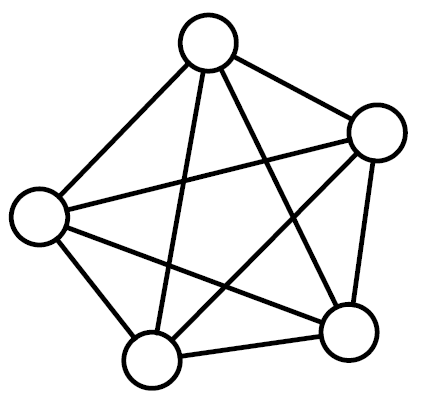
\includegraphics[scale=0.5]{hop.png}
   
   
   }


   \frame{
      \frametitle{The Hopfield model}
      \begin{itemize}
         \item Consists of $N$ nodes $s_i$
      \end{itemize}
   }

   \frame{
      \frametitle{The Hopfield model}
      \begin{itemize}
         \item Consists of $N$ nodes $s_i$
         \item Completely recurrent
      \end{itemize}
   }
   \frame{
      \frametitle{The Hopfield model}
      \begin{itemize}
         \item Consists of $N$ nodes $s_i$
         \item Completely recurrent
         \item Symmetrical: $w_{ij} = w_{ji}$
      \end{itemize}
   }
   \frame{
      \frametitle{The Hopfield model}
      \begin{itemize}
         \item Consists of $N$ nodes $s_i$
         \item Completely recurrent
         \item Symmetrical: $w_{ij} = w_{ji}$
         \item Can be used as an associative memory
      \end{itemize}
   }
   
   \frame{
      \frametitle{The Hopfield model}
   }


\section{} 
   \subsection{Lists I}
   \frame{\frametitle{unnumbered lists}
   }

   \frame{\frametitle{lists with pause}
   }

   \subsection{Lists II}
   \frame{\frametitle{numbered lists}
   }

   \frame{\frametitle{numbered lists with pause}

   }

\end{document}

